\documentclass[fleqn]{article}

\usepackage[margin=2.5cm, headheight=23pt]{geometry}
\usepackage{graphicx}
\usepackage{mathtools}
\usepackage{amsmath}
\usepackage{amsfonts}
\usepackage{colortbl}
\usepackage{empheq}
\usepackage[shortlabels]{enumitem}
\usepackage{caption}
\usepackage{hyperref}
\captionsetup[figure]{labelformat=empty}
\usepackage{subcaption}
\captionsetup[subfigure]{labelformat=empty}

\usepackage{color}

\definecolor{dkgreen}{rgb}{0,0.6,0}
\definecolor{gray}{rgb}{0.5,0.5,0.5}
\definecolor{mauve}{rgb}{0.58,0,0.82}
\definecolor{mauve}{rgb}{1.0,0,0}

\hypersetup{
    colorlinks = true,
    linkcolor=blue,
    urlcolor=cyan,
}


\title{HSE Quick Start Guide}


\begin{document}

\setlength{\parindent}{0cm}

\maketitle

%%%%%%%%%%%%%%%%%%%%%%%%%%%%%%%%%%%%%%%%%%%%%%%%%
\section{Log in to HSE}
%%%%%%%%%%%%%%%%%%%%%%%%%%%%%%%%%%%%%%%%%%%%%%%%%

\begin{itemize}

    \item Open a browser an go to the page \href{http://www.robix-projects.org/hse}{[address of the deployed application]}.

    \item Log in using your personal credentials given to you or the default username \emph{admin} and password \emph{admin}.

\end{itemize}

At this point you see the page shown below. The view contains a list of the existing experiments, and a ``+'' button
for creating new experiments.

\begin{figure}[h!]
\centering
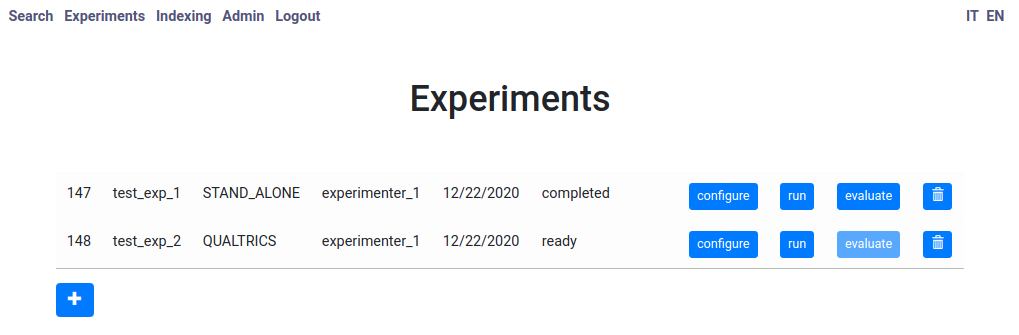
\includegraphics[width=0.7\textwidth]{img/expMain}
%\caption{Typical usage workflow}
%\label{fig:usage}
\end{figure}

%%%%%%%%%%%%%%%%%%%%%%%%%%%%%%%%%%%%%%%%%%%%%%%%%
\section{Define an Experiment}
%%%%%%%%%%%%%%%%%%%%%%%%%%%%%%%%%%%%%%%%%%%%%%%%%

Upon clicking the ``+'' button at the bottom of the experiments list the following popup appears: 

\begin{figure}[h!]
\centering
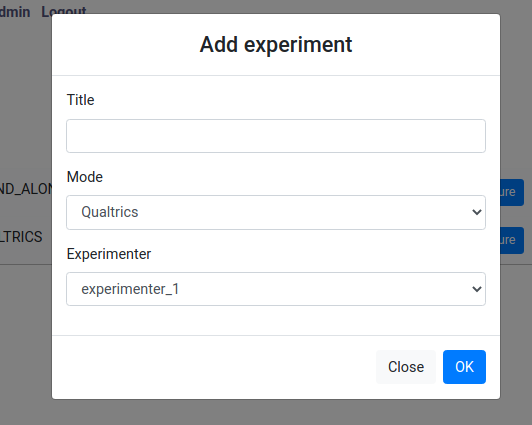
\includegraphics[width=0.3\textwidth]{img/expCreate}
\end{figure}

Set a title for the experiment, and make sure the the mode is set to ``Qualtrics'' and the correct experimenter is selected.
If no experimenter is defined yet, you may create one in the ``Àdmin'' section. 
After clicking ``OK'', a line representing the new experiment is added to the list on the main page.

\begin{figure}[h!]
\centering

\includegraphics[width=0.9\textwidth]{img/expDetail1}
\end{figure}

The leftmost number (302 in the example) is the experiment's id to be used later, when configuring the related \emph{Qualtrics} survey. 

%%%%%%%%%%%%%%%%%%%%%%%%%%%%%%%%%%%%%%%%%%%%%%%%%
\section{Configure the Experiment}
%%%%%%%%%%%%%%%%%%%%%%%%%%%%%%%%%%%%%%%%%%%%%%%%%

Upon clicking the ``configure'' button in the line of the newly defined experiment the following page appears:

\begin{figure}[h!]
\centering
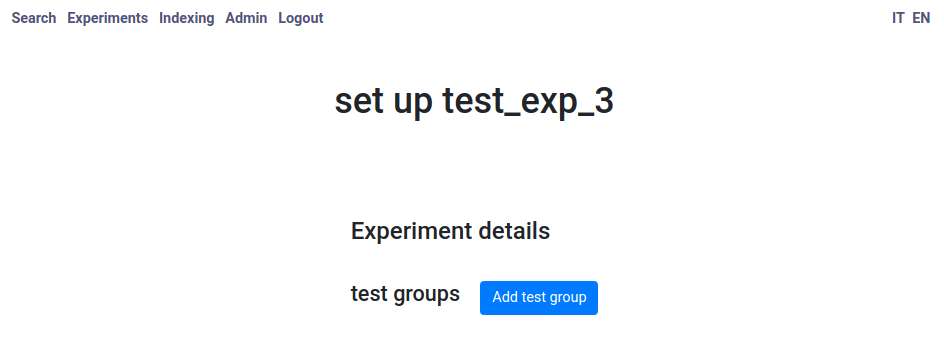
\includegraphics[width=0.7\textwidth]{img/expSetup1}
\end{figure}

At this point you can add the test groups your experiment is supposed to consider by clicking the ``Add test group'' button and
setting a name for each group. The number in square brackets right to each group's name (303 and 304 in the example) is its id to be used later, when configuring the related \emph{Qualtrics} survey.

\begin{figure}[h!]
\centering
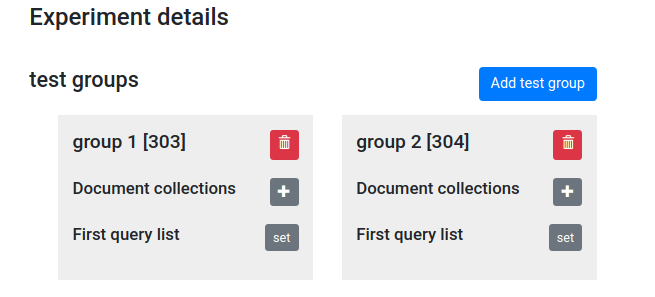
\includegraphics[width=0.7\textwidth]{img/groups1}
\end{figure}

For each defined test group you need to select at least one document collection, and optionally
one collection to be shown in response to the participant's first query.

\begin{figure}[h]
     \centering
     \begin{subfigure}[b]{0.4\textwidth}
         \centering
         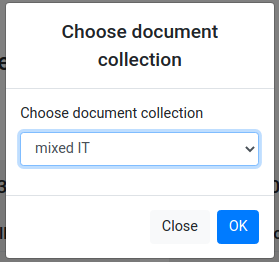
\includegraphics[width=.7\linewidth]{img/groups2}
     \end{subfigure}
     \begin{subfigure}[b]{0.4\textwidth}
         \centering
         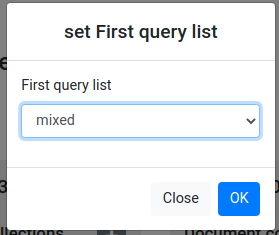
\includegraphics[width=.8\linewidth]{img/groups3}
     \end{subfigure}
\end{figure}

\newpage

%%%%%%%%%%%%%%%%%%%%%%%%%%%%%%%%%%%%%%%%%%%%%%%%%
\section{Configure the Qualtrics Survey}
%%%%%%%%%%%%%%%%%%%%%%%%%%%%%%%%%%%%%%%%%%%%%%%%%

The following points assume you are using a previously configured survey. If you need to set up a new survey from scratch,
please refer to the ``HSE Setup and Usage Guide''.

\begin{enumerate}

    \item In the survey flow interface set the experiment id in the first \emph{embedded data} element:       
        
        \begin{figure}[h!]
        \centering
        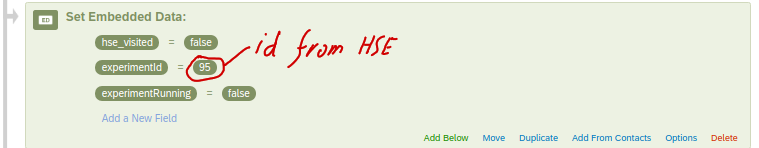
\includegraphics[width=0.7\textwidth]{img/qflow1}
        \end{figure}

    \item Set an \emph{embedded data} element for each test group within the \emph{Randomizer} element:

        \begin{figure}[h!]
        \centering
        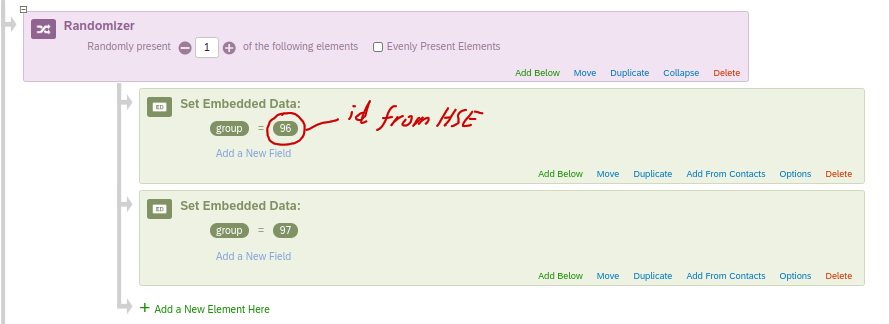
\includegraphics[width=0.7\textwidth]{img/qflow4}
        \end{figure}

\end{enumerate}

%%%%%%%%%%%%%%%%%%%%%%%%%%%%%%%%%%%%%%%%%%%%%%%%%
\section{Run the Experiment}
%%%%%%%%%%%%%%%%%%%%%%%%%%%%%%%%%%%%%%%%%%%%%%%%%

When everything is configured you can access the run interface and start the experiment.

\begin{figure}[h!]
\centering
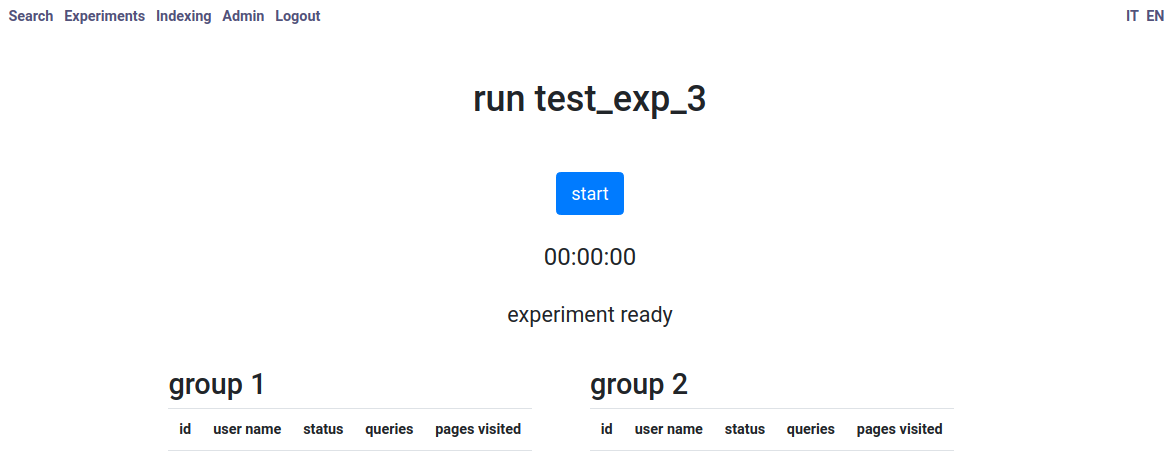
\includegraphics[width=0.7\textwidth]{img/expRun1}
\end{figure}

At this point you can distribute your survey a and wait for the participants to complete it, and stop the experiment
when enough data has been collected.

\newpage

%%%%%%%%%%%%%%%%%%%%%%%%%%%%%%%%%%%%%%%%%%%%%%%%%
\section{Evaluate the Experiment}
%%%%%%%%%%%%%%%%%%%%%%%%%%%%%%%%%%%%%%%%%%%%%%%%%

After having stopped the experiment, its evaluation page becomes available. Here you can have a look at a summary
of the collected data and export the results:

\begin{figure}[h!]
\centering
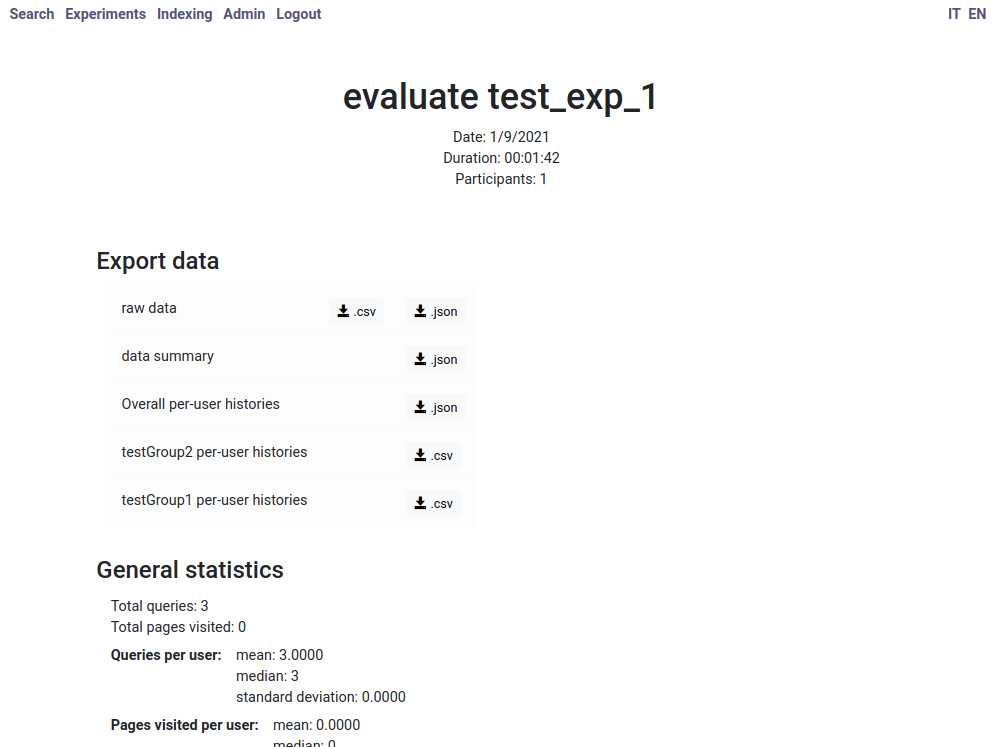
\includegraphics[width=0.9\textwidth]{img/expEval}
\end{figure}
 

\end{document}















